																																											\documentclass{article}
\usepackage[utf8]{inputenc} % Allow using of åäö, etc.
\usepackage{graphicx} % Add pictures.
\usepackage{verbatim} % Add multiline comments.

% comment about something
\author{Mikael Grön, Anssi Moisio, Visa Koski, Lassi Knuuttila}
\title{Q-learning Project Documentation - C++ ELEC-A7150}
\date{\today}

\begin{document}

\maketitle

\tableofcontents
\newpage

\section{Overview}
Main functionalities of this Q-learning implementation include:
\begin{itemize}
  \item Support for a crawler creature that has an arm with two joints. The
  crawler's purpose is to crawl to the right in a 2D-world using its arm.
  \item Many crawlers learning at the same time, in different threads.
  \item A command line user interface from which user can pause learning and
  save the Q-table.
  \item Crawlers can share their knowledge with other crawlers to speed up
  the learning process.
\end{itemize}

The crawler looks like this:

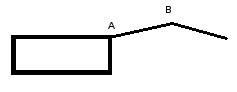
\includegraphics[width=0.8\textwidth]{simple_agent}

We could not get the graphics Box2D's Testbed to work. Problems arose with
the GLUT library lacking compatibility with threading.

A plan-B was to visualize the Qtable with Cairo graphics library which we
configured, but we didn't have time to implement the visualization.

As a substitute for graphics, the command line interface prints out the
crawlers’ locations and speeds at regular intervals. It can be observed
from the prints that a crawler learns a maneuver by which it acquires some
top speed. After acquiring a top speed, the movement is stable (velocity is
constant) if the exploration factor is set to a low value, so that the crawler
does not make random actions.

The original plan was to make the programm support many kinds of learning
creatures. This is the case for some of the classes (Qtable, AgentManager)
but not all. AgentLearner class has support for crawlers with one or two joints
and the Simulation class supports only crawlers with two joints. The finished
program is thus compatible with a crawler that has two joints, but compatibility
for different kinds of crawlers could be implemented with relatively small
changes, which we did not have time for.

\subsection{Configuration-file}
The support for many kinds of learning Agents is visible also in the
configuration-file, where the plan was to have the option to change what
Agent you run, without changing source-code. Because of obstacles and
not having time, the only things you can modify are the number of Agents
per run, and initializing the Agent(s) QTable from a saved file.

\subsection{Evolution}
When running more than one Agent evolution is used. This means that the
Q-Learning algorithms variables differ some from the first Agents, which
has always the same variables.
All Agents in a run form the current generation. When one of the Agents
reaches to a certain distance the goal, then this Agent is the fittest. All
other Agents will copy the fittest Agents QTable into theirs, and every Agent
teleports to the starting position. Then the next generation tries to
reach the goal. And so on.


\section{Software structure}
The main divide of the program is: learning and simulation. The
simulation and the learning parts communicate with each other mainly by the
learning part telling the simulation to do an action. The simulation will then
simulate the action, returning the new simulated change of the agent to the
learning part. The learning part evaluates the simulated change, determining
what the reward for the performed action was, updating the Q-value.

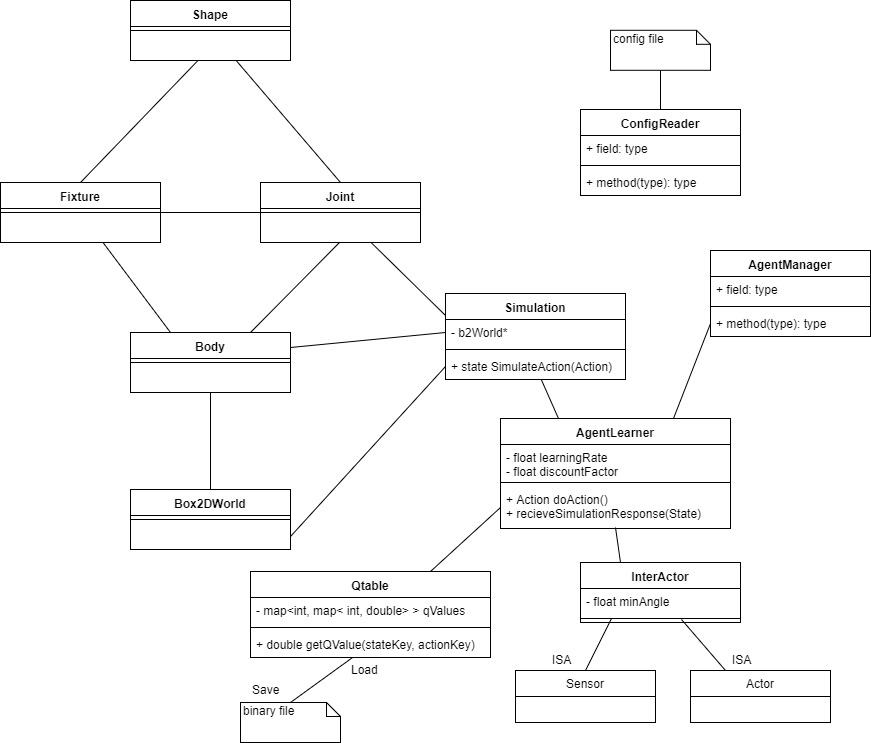
\includegraphics[width=1\textwidth]{c++UML}

\subsection{Q-learning}
The learning process takes place in the AgentLearner class.
An object of the AgentLearner
class uses a Qtable object to store and access the Q-table. A Qtable object
has a two-dimensional map structure for storing the Q-values of each
state-action pair. A map structure is used instead of, for example,
a vector structure which was the original plan, so the size of
the Q-table is possible to scale up without the access time increasing.

The Qtable class is supports dynamic creation and an object is initialized
from a vector of actors and a vector of sensors. Initializer needs
the number each actor's possible actions and the number of each
state-detecting sensor's possible states. Qtable is a map of
state-maps that contain actions for that state. The size of the Qtable
will be states * actions. If an agent has, for example, three actors
with 3, 2 and 2 possible actions, for each state there is
3 * 2 * 2 = 12 possible actions. If three state-detecting sensors can
detect each 10 different states, the total number of states is
10*10*10 = 1000. This would make a Qtable of a size 1000 * 12.

The Qtable class has functions for finding the best action and finding
the optimal Q-value for a state of the crawler. These are used in the
learning process to update the Q-values.

The AgentLearner needs to convert the state of the learning crawler to a key
for the Qtable object. The states are quantisized from the continuous states
that the crawler can have in the simulation. StateKeys are in the format
int stateKey = 141315, where each sensor's
state is represented by two digits (14, 13, 15). Sensors' states are
in the range 1...quantizationSteps. ActionKeys are in the format
int actionKey = 30302 where each sensor's
state is represented by two digits (3, 3, 2). Actors' moves are
enumerations: 0 still, 1 counterclockwise and 2 clockwise and 1 is
added to them so the key cannot be 000000.

\subsection{Simulation}
The simulation was meant to be done with Box2D's Testbed framework that 
offered some physics demos. We made a new test that simulated our crawler
and the user could control it with WASD-keys (demoed in the mid-term meeting).
The problems started when we tried to combine it with the Q-learner as the
Testbed paused the Q-learner thread. This was because the OpenGL library GLUT
didn't seem to be compatible with multiple threads. So we discarded our work on
Testbed and started investigating Cairo graphics library but our time was running out
so we didn't implement it in our project. 

\subsection{Thread management}
The AgentManager-class controlls the treads and their running trough
atomic-booleans and mutexes. Every threads task is the AgentTask-function
in agent\_manager.cpp. AgentManager listens on the users and AgentTasks
inputs.

\subsection{User Interface}
Because there was problems with our graphics library, we do not have a GUI.
The program is started from the commandline, where controlls listed
to controll the program when it is running.

The Agent(s) location in the simulation is visible on the commandline as:

"65k: Agent\_0 V=127 X=6418.52"

\textbf{Meaning:}

\begin{tabular}{ll}
65k                     & 65 thousand actions executed \\
Agent\_0                & Line conserns Agent number 0 \\
V=127                   & Agents velocity in simulation units per 5k actions\\
X=6418.52               & Agents location in simulation units\\
\end{tabular}


\section{Instructions for using the program}

\subsubsection{Build}
Cmake creates the Makefiles, and make uses the Makefiles to build the project.

\begin{itemize}
  \item Install required packages if they're not installed already
  \textbf{sudo apt install cmake}

  \item Move to the build folder in the q-learning-9 folder.
  \textbf{cd q-learning-9/build/}

  \item Create Makefile.
  \textbf{cmake ..}
\end{itemize}

Build targets can be listed, built together, built separately and removed:

\begin{itemize}
  \item List targets that can be built. \textbf{make help}

 \item Compile everything. \textbf{make} or \textbf{make all}

 \item Compile main. \textbf{make main}

 \item Compile tests. \textbf{make qtests}

 \item Remove compiled targets. \textbf{make clean}

 \item The executable compiled targets will be in the build folder as:
  \textbf{main} and \textbf{qtests}
\end{itemize}

\subsubsection{Running}
The program is run from the built file: build/main.
The program is optionally configured from the file: src/configAgent.config.
In the config-file you can change how many Agents are running and
an optional file for a saved qtable-file.


\section{Testing}
Testing is done with unittest trough googletest.
The test are built as the "qtests"-buildtarget in cmake.
The built test are run from file: build/qtests.
Valgrind has been used from time to time, but it is not automated.


\section{Worklog}

\subsection{Mikael}
My main area I worked on was the planning, building, AgentManager,
Interactor and the configuration-file. I helped also partly with nearly all
other parts.
A detailed log of what I worked on can be found from the GitLab-commit-history,
and the time spent was not recorded.


\subsection{Visa and Lassi}
Our area was implementing the Box2D, simulation and graphics. However, as we didn't
get the graphics to work, we had to discard them.

\subsection{Timeline}

\subsubsection{Week: Nov 6th to 12th}
Anssi:
Configured the programming environment, i.e., linux virtual machine.
Planned the learning classes; what functions they will need and what
member data they will use. Planned the distribution of roles between
Mikael and myself, as we are the group members that implement the learning
algorithm.
15 hours

Visa: 
studied box2d.
2 hours

Lassi:
Set up the virtual machine. Studied how Box2D works
5 hours

\subsubsection{Week: Nov 13th to 19th}
Anssi:
Continued planning the project, made the UML picture for the plan.
3 hours

Visa
virtual machine set up, started learning box2d and worked on plan
and UML with lassi 
8 hours

Lassi:
Continued watching educational videos on Box2D. Created the Simulation 
part of the UML and project plan with Visa. 
10 hours

\subsubsection{Week: Nov 20th to 26th}
Anssi:
Planned the Q-learning implementation with Mikael and started coding.
My responsibilities are the AgentLearning and Qtable classes.
10 hours

Lassi:
Started implementing Box2D. Busy week from outside the course.
5 hours

\subsubsection{Week: Nov 27th to Dec 3rd}
Anssi:
Implemented functions in the Qtable class and in the Agent class and
re-named the Agent class as AgentLearner. Made tests for these functions.
Changed Q-table data structure from vectors to maps.
30 hours

Visa:
started working on Box2d. implemented testcrawler to testbed.
20 hours

Lassi:
After a lot of trial and error, Visa and I got the simulation to a point 
where one could control the crawler with keyboard. We used a testbed from 
Box2D and decided to keep it so that the Q-learner would control the testbed.
25 hours.

\subsubsection{Week: Dec 4th to 10th}
Anssi:
Implemented functions in the Qtable class and in the Agent class, for
converting actions and states to keys for the Q-table map and choosing
the Action. Also for saving and loading Q-table from a file.
25 hours

Visa:
started work on simulation class, majority of work went trying to get crawler
position that caused segfault. Added lot of crawler properties and debug to testbed
that we tried to combine to Qlearner with Lassi.
20 hours

Lassi: Tried to combine the Box2D testbed and the Q-learner with no success
20 hours

\subsubsection{Week: Dec 11th to 17th}
Anssi:
Finalized AgentLearner class and Qtable class and implemented the
Simulation class with Visa. Tried to visualize the Q-table with
Cairo graphics library, but didn’t have time to finish. Debugged
and optimized  the learning process.
26 hours

Visa:
implemented the Simulation class with Anssi. Lot of debugging was done with
crawler, box2dworld and parameters. Added comments to crarify whenever needed
28 hours

Lassi:
The week was very eventful and I didn't have that much time for the project.
Stripped the testbed off of all OpenGL-components. After that we decided not
to use the testbed at all.
3 hours

\subsubsection{Week: Dec 18th}
Anssi:
Wrote the documentation.
6 hours

Visa:
documentation.
3 hours

Lassi:
Created the simulation part of the documentation
2 hours:

\end{document}
